\label{sec:metrics}

Once defined the coding schemes behavior in terms of encoding
and decoding, we proceed to describe the metrics considered in our study.
The goodput is a measure for the effective processing speed since it
excludes protocol overhead but considers all delays related with
algorithmic procedures, field operations, hardware processing, multicore
coordination (where it applies), etc. Moreover, both encoding and decoding
goodput permit to observe if coding is a system-block that limits the
end-to-end performance. If a system presents a low goodput, this will
affect the \ac{QoE} of delay-intolerant applications for the end user.
For example, mobile user applications are typically delay-intolerant.
Furthermore, \ac{Raspi} processors are based in the \ac{ARM} architecture
which is the same as in mobile devices such as smartphones or tablets.
Thus, the \ac{Raspi} might be used as an experimental tool to get an
estimate of a mobile device processing capability which is easy-deployable
and at a much lower cost than a smartphone.

To complement our study, we review the energy consumption of the \ac{Raspi}
since this platform is deployed at a large scale in scenarios where (i)
energy is constrained to the lifetime of the device battery and (ii) the
devices could be established in locations that are unavailable for
regular maintenance. Typical use cases of this type of scenarios are
sensor applications where devices are positioned for measurement retrieval
without any supervision for large periods fo time.

\subsection{Goodput}
We consider the goodput defined as the ratio of the useful delivered
information at the application layer and the total processing time. We focus
on the goodput considering only the coding process, i.e. we assume that
the application data has been properly generated before encoding and
also correctly post-processed after decoding. In this way, we define
the goodput for either an encoder or a decoder as follows:
%
\begin{align} \label{eq:goodput}
R_{proc} = \frac{gB}{T_{proc}} ~ [\mathrm{Bytes/second}]
\end{align}
%
In \eqref{eq:goodput}, $B$ and $g$ are the packet and generation size
as defined previously and both represent the data to be processed. For
goodput measurements, we are concerned in quantifying the processing time
for either encoding or decoding $g$ \ac{l.i.} packets. Thus, $T_{proc}$ is
the processing time required for this processing. In the next subsections, we
define two time bechmarks available in \cite{soerensen2016sparse}.
The purpose of the benchmarks is to quantify the processing time for
any of the coding schemes considered in Section \ref{sec:schemes}.

\subsubsection{Encoding Benchmark}
Fig. \ref{fig:enc_goodput_benchmark} refers to the benchmark setup
made for measuring the encoding processing time. The time benchmark
is divided in two parts. In the first part, called a \textit{pre-run},
we quantify the amount of \textit{transmitted} coded packets from an
encoder (named 1 in Fig. \ref{fig:enc_goodput_benchmark}) required for
decoding in a single encoder-decoder link with no packet erasures
for a defined configuration of coding scheme, coding parameters and
amount of feedback. In the case of \ac{TSNC}, we also record the
points where a feedback was received from the decoder. The purpose of
the pre-run is to predict how an encoder should behave with a given
seed within its random number generator. This part of the benchmark is
not regarded as a measurement.

In the second part which is the actual \textit{simulation}, a reseted
encoder (2 in Fig. \ref{fig:enc_goodput_benchmark}) is given the same
seed as in the pre-run and then we measure the time from which the
process start until we reach the amount of transmitted packets in the
pre-run. Then, this measurement is stored as the encoder $T_{proc}$
for this generic configuration.

\begin{figure}[ht!]
\centering
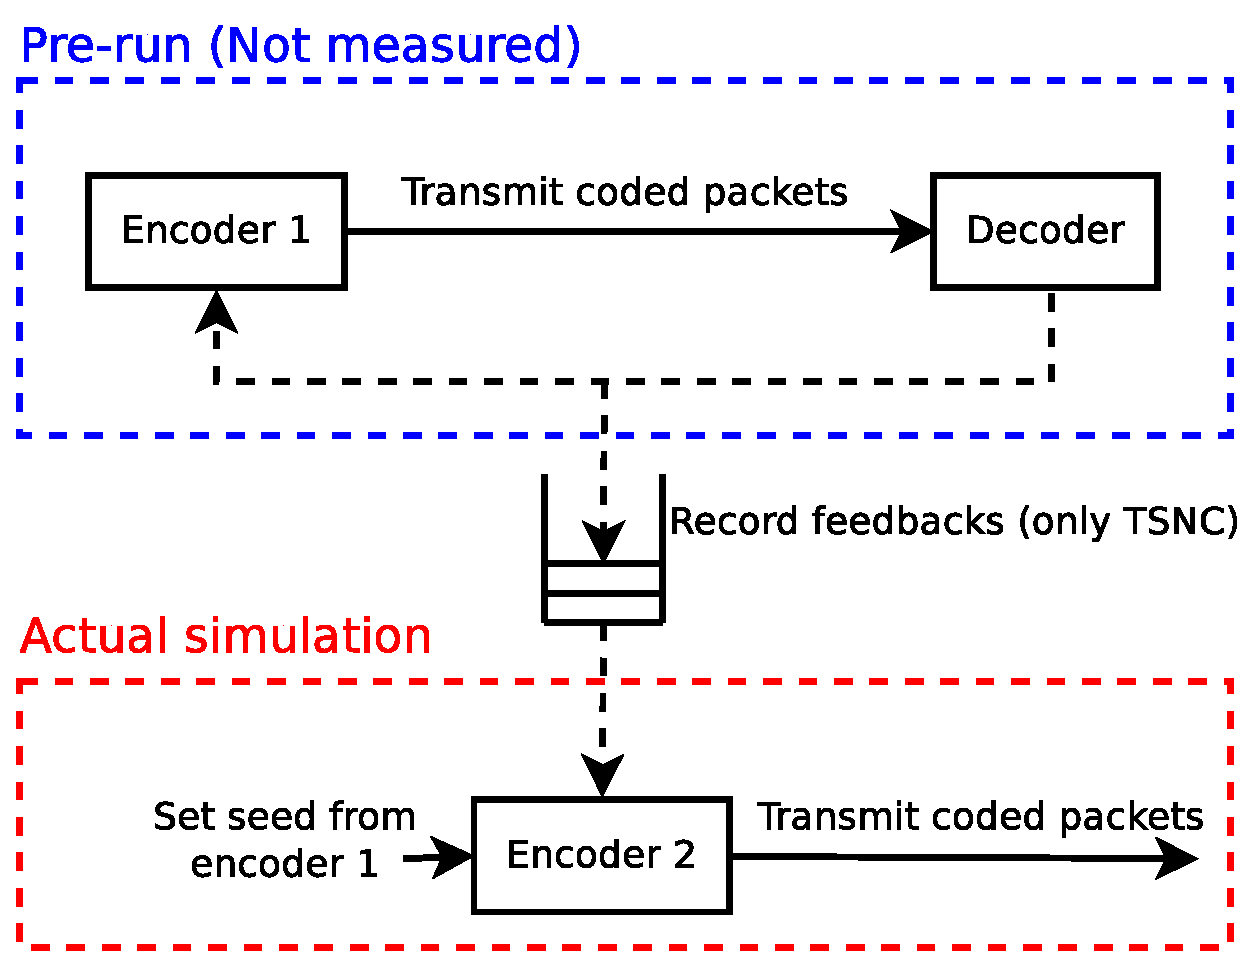
\includegraphics[width=0.6\textwidth]{images/measure_encoder.eps}
\caption{Encoding goodput benchmark}
\label{fig:enc_goodput_benchmark}
\end{figure}

\subsubsection{Decoding Benchmark}
Fig. \ref{fig:dec_goodput_benchmark} shows the benchmark setup
for measuring the decoding processing time. The time benchmark
is divided in two parts as its encoding counterpart, e.g. a pre-run
and the actual simulation. However, some differences occur.

In the pre-run, we still quantify the amount of transmitted coded
packets from encoder 1. Notice that we include the feedback case because
it is necesary for the \ac{TSNC} scheme. However, now we store
the \textit{transmitted packets} instead. The reason being
that we want to feed the decoder with the same packets in the same
order. Later, in the actual simulation, an encoder (2 in Fig.
\ref{fig:dec_goodput_benchmark}) is given the same packets in the same
order from the pre-run and then we measure the time from which the
process start until the decoder finishes to retrieve the original
packets. Finally, this measurement is saved as the decoder $T_{proc}$
for this general configuration.

\begin{figure}[ht!]
\centering
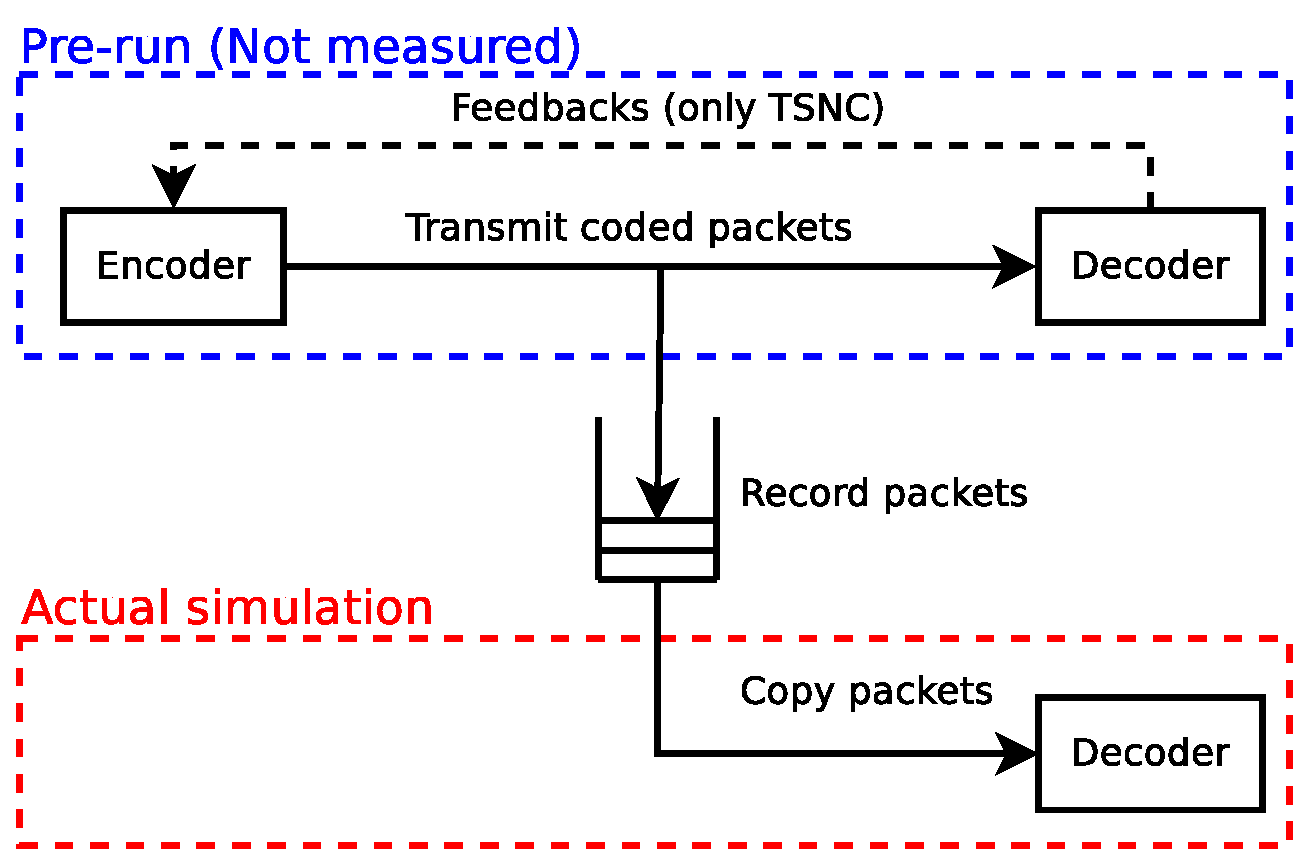
\includegraphics[width=0.6\textwidth]{images/measure_decoder.eps}
\caption{Decoding goodput benchmark}
\label{fig:dec_goodput_benchmark}
\end{figure}

\subsection{Energetic Expenditure}
\label{sec:energy_metrics_methods}
In large-scale networks where several \ac{Raspi}s might be deployed,
both average power and energy per bit consumption of the devices are
relevant parameters that impact in the network performance for a given
coding scheme. Hence, we consider a study of these energy expenditure
parameters for the encoding and decoding. We define these metrics
and propose a setup to measure them.

The average power specifies the rate at which energy is
consumed in the \ac{Raspi}. Thus, for a given energy value in the device
battery without any external supplies, this metric permits to infer the amount
of time for which the \ac{Raspi} can operate autonomously before draining
out its battery. For the energy per bit consumption, it indicates how
much energy is expended to effectively transmit or receive 1 bit of
information taking into account the encoding or decoding operations
respectively.

For our energy measurement campaign, we automate the setup presented
in Fig.~\ref{fig:measurement_setup} to sequentially run a series of
simulations for a given configuration of a coding scheme and its parameters,
to estimate the energic expenditure in both of our \ac{Raspi}
models. The energy measurement setup goal is to quantify the power
consumption of the \ac{Raspi} over long periods of processing time to
obtain accurate results. A representative sketch of the setup is shown
in the computer monitor in Fig.~\ref{fig:measurement_setup}.

The energy measurement setup presents a \ac{Raspi} device whose power
supply is an Agilent 66319D \ac{DC} source, instead of a conventional
power chord supply.   To compute the power, we just need to measure
the current since the \ac{Raspi} feeds from a fixed input voltage of $5V$
set by the Agilent device, but its current consumption is variable.
Hence, the measured variable is the current consumed by the device for
this fixed input voltage. The output of the measurements
are later sent to a workstation where the raw measurement data is processed.

\begin{figure}[ht!]
\centering
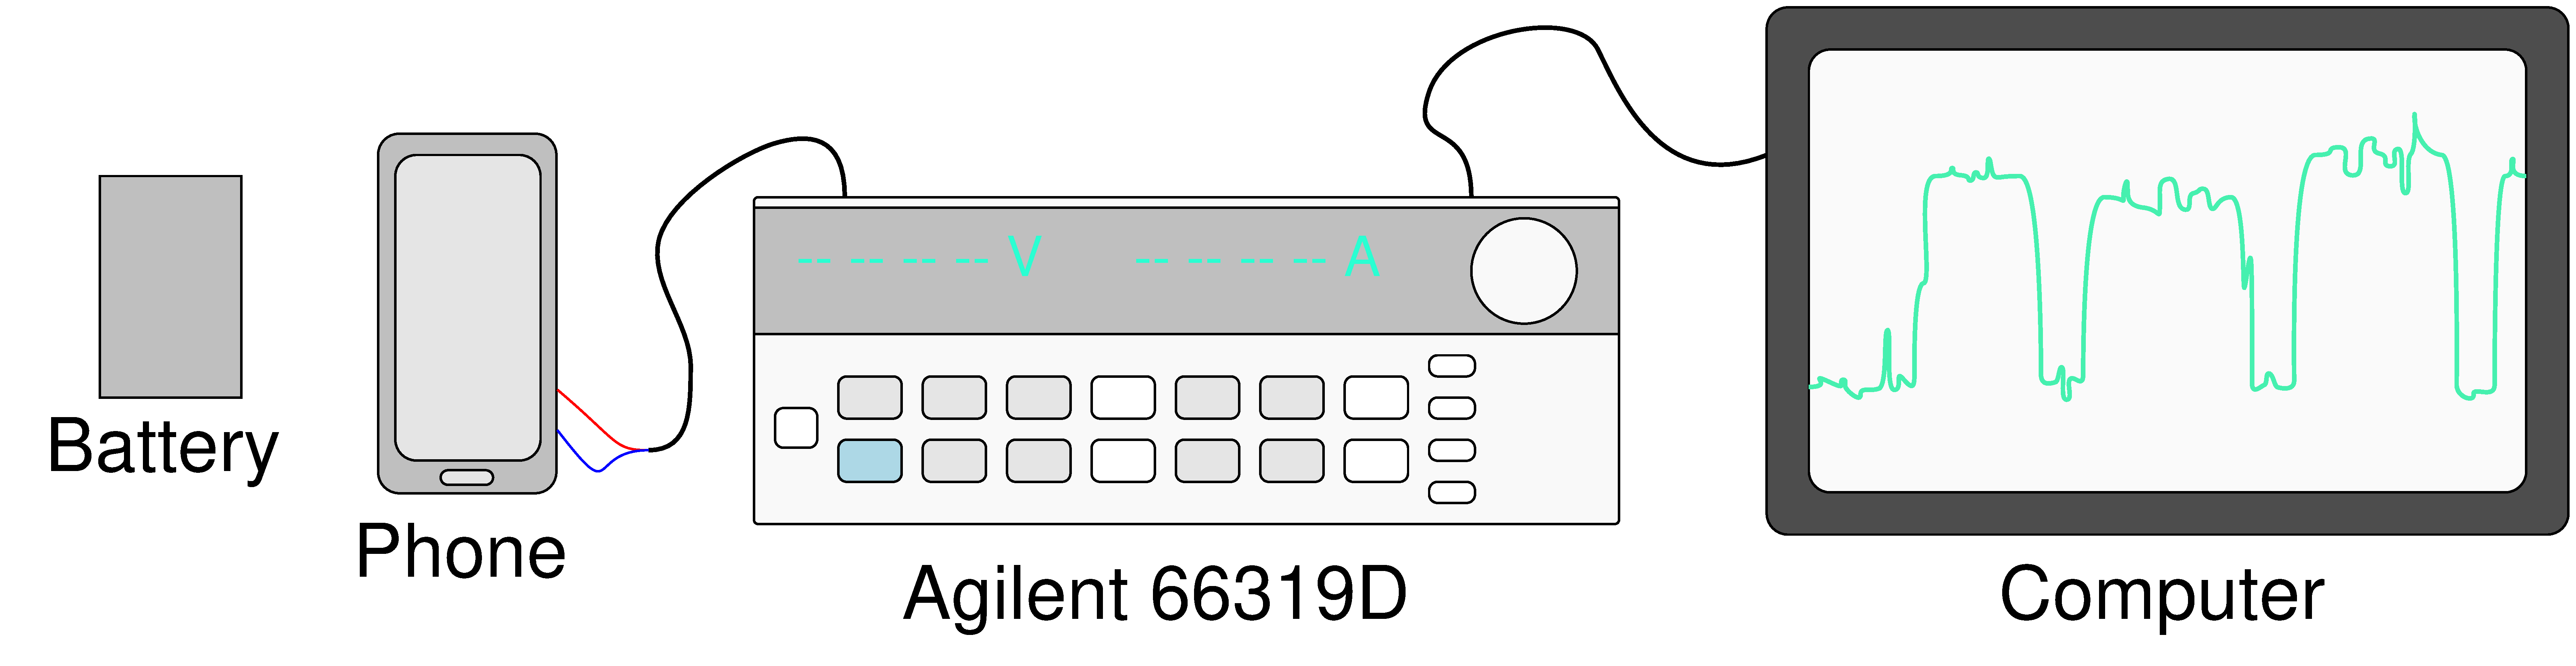
\includegraphics[width=0.7\textwidth]{images/measurement_setup.eps}
\caption{Energy measurement setup}
\label{fig:measurement_setup}
\end{figure}

To identify each experiment, we classified the electrical current samples
into two groups based on the magnitude. In our measurements, the groups to
be reported are the idle current $I_{idle}$ and the processing current
$I_{proc}$. The former is the current the \ac{Raspi} requires while in idle
state, meaning that no processing is being carried. The latter stands for
the current needed during the encoding or decoding processing of the packets.
Measurements are taken either when $I_{idle}$ or $I_{proc}$ are observed.
For the processing currents, its current measurements are made while the
goodput benchmarks are running for a given configuration of a coding scheme
with its parameters. For each configuration, $10^3$ simulations from the
goodput benchmarks are carried during the period of time where $I_{proc}$
occurs. We remark that a simulation is the conveying of $g$ \ac{l.i.} coded
packets. Finally, for each configuration, each set of current measurements is
enumerated to map it with its average power value and the corresponding goodput
measurements. At post-processing, from the average power expenditure and the
results from the goodput measurements it is possible to extract the energy
per bit consumption. We elaborate further on this post-processing in the
next subsections.

\subsubsection{Average Power Expenditure}
To extract the average power for a given configuration in our setup, we
first calculate the average current in each the idle state $I_{idle,avg}$
and the processing state $I_{idle,avg}$ for all the available sample for
the given configuration. Regardless of the current type, the average value
of the sample set of a given number of samples $N_s$ is:
%
\begin{align} \label{eq:avg_current}
I_{avg} = \frac{1}{N_s}\sum_{k=1}^{N_s} I_{k}  ~[\mathrm{Amperes}]
\end{align}
%
With the average current from \eqref{eq:avg_current}, we compute the average
current used for processing with respect to the idle state, by substracting
$I_{idle,avg}$ from $I_{proc,avg}$. Then, the result is multiplied by the
supply voltage to obtain the average power during the considered configuration,
given as:
%
\begin{align} \label{eq:avg_power}
P_{avg} = V_{supply}(I_{proc,avg} - I_{idle,avg}) ~[\mathrm{Watts}]
\end{align}
%
\subsubsection{Energy per Bit Consumption}
To get this metric for a given configuration, we simply express the energy
as the product of the average power by the processing time $T_{proc} [sec/byte]$
obtained from the goodput measurement for the same configuration. In this way, we can
relate the processing time with the goodput, the packet and the generation size
as shown:
%
\begin{align} \label{eq:energy_per_bit}
E_b = P_{avg} T_{proc,bit} = P_{avg} \times \frac{T_{proc}}{8gB} = \frac{P_{avg}}{8R_{proc}} ~[\mathrm{Joules}]
\end{align}
%
